% !TEX TS-program = xelatex
% !BIB TS-program = bibtex
\documentclass[12pt,letterpaper]{article}
\usepackage{style/dsc180reportstyle} % import dsc180reportstyle.sty
\newcommand{\lmul}{$\mathcal{L}$-Mul\xspace}

%%%%%%%%%%%%%%%%%%%%%%%%%%%%%%%%%%%%%%%%%%%%%%%%%%%%%%%%
%%%% Title and Authors
%%%%%%%%%%%%%%%%%%%%%%%%%%%%%%%%%%%%%%%%%%%%%%%%%%%%%%%%

\title{Multiplication is Not What You Need: Efficient Floating Point Multiplication on FPGAs}

\author{Kai Breese \\
  {\tt kbreese@ucsd.edu} \\\And
  Lukas Fullner \\
  {\tt lfullner@ucsd.edu} \\\And
  Justin Chou \\
  {\tt jtchou@ucsd.edu} \\\And
  Katelyn Abille \\
  {\tt kabille@ucsd.edu} \\\And
  Rajesh Gupta \\
  {\tt rgupta@ucsd.edu} \\}

\begin{document}
\maketitle

%%%%%%%%%%%%%%%%%%%%%%%%%%%%%%%%%%%%%%%%%%%%%%%%%%%%%%%%
%%%% Abstract and Links
%%%%%%%%%%%%%%%%%%%%%%%%%%%%%%%%%%%%%%%%%%%%%%%%%%%%%%%%

\begin{abstract}
    Efficient floating point operations are a significant challenge in large neural networks and other computationally intensive machine learning algorithms, where energy consumption and latency are key constraints. In this report, we present an implementation of the linear-complexity multiplication (\lmul) algorithm designed to approximate floating point multiplication using addition \citep{luo2024addition}. By leveraging this approximation, \lmul achieves high precision with significantly lower computational cost than traditional floating point multiplication methods. Our approach aims to further deploy this method on field-programmable gate arrays (FPGAs), offering a reduction in energy consumption and processing time. Our goal of deployment to FPGAs will provide practical benchmarking of the algorithm applied closer to the hardware level, going beyond implementation on existing GPU hardware.
\end{abstract}

\begin{center}
% Website: \url{https://abc.github.io/} \\ % to  be added quarter 2
Code: \url{https://github.com/ninjakaib/hardware-accelerators}
\end{center}

\maketoc
\clearpage

%%%%%%%%%%%%%%%%%%%%%%%%%%%%%%%%%%%%%%%%%%%%%%%%%%%%%%%%
%%%% Main Contents
%%%%%%%%%%%%%%%%%%%%%%%%%%%%%%%%%%%%%%%%%%%%%%%%%%%%%%%%

\section{Introduction}

As modern artificial intelligence (AI) systems grow in scale and complexity, their computational processes require increasingly large amounts of energy. Notably, ChatGPT required an estimated 564 MWh per day as of February 2023. In comparison, the cost of two days nearly amounts to the total 1,287 MWh used throughout the training phase, implying that energy consumption in the inference phase is considerably more expensive in the long term \citep{de2023growing}. Such patterns go beyond models like ChatGPT, as Google also reports that 60\% of its ML energy usage was for inference \citep{carbonfootprint2022}. Beyond monetary costs, the extensive energy consumption of large language models (LLMs), neural networks, etc. is now raising concerns about environmental impacts. Thus, the need for new hardware to efficiently handle inference is essential. Addressing this challenge, we aim to investigate a new approach by building off of the existing linear-complexity multiplication (\lmul) algorithm developed by \cite{luo2024addition}, which achieves high precision while reducing computational overhead. Our study proposes deployment on FPGAs and the potential for ASIC implementation to amplify these benefits. Our advancements suggest that \lmul could play a critical role in optimizing neural network efficiency, ultimately contributing to more energy-efficient AI development.


\subsection{Prior Work}

Already, we have seen the increasing development of specialized AI chips designed to optimize training and inference efficiency. Google's Tensor Processing Unit (TPU), for example, leverages a systolic array architecture to accelerate tensor operations, particularly matrix multiplication.\footnote{\url{https://cloud.google.com/blog/products/ai-machine-learning/an-in-depth-look-at-googles-first-tensor-processing-unit-tpu}} AWS Inferentia2 delivers 4x higher throughput, 10x lower latency, and 10x memory bandwidth than its original model with support for up to 190 TFLOPS of FP16 performance.\footnote{\url{https://aws.amazon.com/ai/machine-learning/inferentia/}} Alongside Intel Gaudi, Groq Language Processing Unit (LUP), and more, the market for new AI hardware continues to grow.

\subsubsection*{Literature Review}

In our exploration of hardware acceleration for machine learning, we reviewed prior domain work by \citep{b182023}, which tested a human activity recognition system on various virtual CPU and GPU configurations. Their results revealed that increasing virtual CPU cores only accelerated the transformer-based model, while the CNN and DNN model’s performance remained constant. They also found no performance gains from increased virtual memory, highlighting that the bottleneck lies in transferring data \textit{from} memory \textit{to} the processor. Their final GPU experiments demonstrated that enhanced parallelism drives performance gains, guiding our study's focus on implementing widely parallel systems to optimize speedup.

To better understand the role of FPGAs, we reviewed neural network acceleration techniques based on FPGA platforms \citep{liu2024review}. The paper gathers current research on FPGA accelerators, covering many topics surrounding design and implementation. It highlights the limitations of FPGAs compared to GPUs, which achieve significant speedups beyond what any FPGA could accomplish due to the incredibly optimized nature of GPUs. The nature of an FPGA operates more similarly to a CPU, whereas GPUs consist of a large field of cores optimized for parallel processing. The paper then describes an interesting take on designing programs for FPGAs, that being an algorithm hardware collaborative optimization method. The goal of this method is to reshape the design methodology from implementing the algorithm, then perform high-level synthesis to convert it to code for the FPGA to instead design code with the processor in mind, and develop the two side by side. This programming paradigm will be very useful as we develop our FPGA implementation.

The final paper we draw upon is where we draw the \lmul algorithm, and as such is where the bulk of our information comes from \citep{luo2024addition}. The core of the algorithm comes from an optimization of the floating point multiplication algorithm that cuts out the multiplication step with floating point addition. The key insight occurred when looking at the steps taken during multiplication: the only multiplication occurring in this algorithm is the multiplication of the mantissa bits, but this can be simplified. The core of the paper is replacing the multiplication term with a discovered offset term $2^{-4}$, found by testing model performance with a variety of terms leading to the lowest error. The algorithm is an approximation, but the error is low enough to not affect model performance and gains the advantage of removing the time-consuming multiplication step and reducing the algorithm to an addition, a subtraction, and an XOR for the sign bit.

\subsection{Data Applications}

Multiplication is already an existing algorithm that is already fast on the processor, so why do we want to accelerate such a basic mathematical process? The reason: time and energy. The vast majority of data science is matrix multiplication operations, so in optimizing that core step, much of a neural network’s runtime is also improved upon. This means optimizing the time leads to faster processing and by extension faster models, leading to faster response times for LMMs and other transformers. And, by lowering the number of operations, the energy requirement goes down, meaning the cost of operating the model goes down.

The second question is: Why are we targeting our implementation to FPGAs instead of to GPUs? GPUs are purpose-built to do math operations at great speed and massively in parallel, and as such seem like a good destination for our optimization. Our goal for an FPGA implementation is to achieve maximal speed up using the algorithm, and while a GPU could run it quickly, running it on an FPGA would allow us to configure the hardware to match our algorithm, maximizing time and energy savings as discussed.


\section{Methods}

\subsection{Background: Framework for Floating-Point Arithmetic}

\subsubsection*{Floating-Point Numbers}

Today, most machine learning models and algorithms use floating-point (FP) tensors, typically in FP32 or mixed-precision formats like FP16 or BF16, to represent their inputs, outputs, and trainable parameters \citep{luo2024addition}. Let's take a look at the basic format of floating-point numbers, starting with OCP 8-bit Floating Point Specification (OFP8).\footnote{\url{https://www.opencompute.org/documents/ocp-8-bit-floating-point-specification-ofp8-revision-1-0-2023-12-01-pdf-1}}

\begin{table}[htbp]
    \caption{OFP8 exponent parameters}
    \label{tab:ofp8_exp}
    \resizebox{0.5\linewidth}{!}{\centering
\begin{tabular}{ccc}
Parameter       & E4M3 & E5M2 \\
\midrule
Exponent bias   & 7    & 15   \\
emax (unbiased) & 8    & 15   \\
emin (unbiased) & -6   & -14  \\
\end{tabular}
}
\end{table}

\begin{table}[htbp]
    \caption{OFP8 value encoding details}
    \label{tab:ofp8_encode}
    \resizebox{.9\linewidth}{!}{\renewcommand{\arraystretch}{1.25}
\centering
\begin{tabular}{lll}
Parameter            & E4M3                        & E5M2                        \\
\midrule
Infinities           & N/A                         & S.11111.00₂                 \\
\hline
NaN                  & S.1111.111₂                 & S.11111.{01, 10, 11}₂       \\
\hline
Zeros                & S.0000.000₂                 & S.00000.00₂                 \\
\hline
Max normal number    & S.1111.110₂ = ±448          & S.11110.11₂ = ±57,344       \\
\hline
Min normal number    & S.0001.000₂ = ±2⁻⁶          & S.00001.00₂ = ±2⁻¹⁴         \\
\hline
Max subnormal number & S.0000.111₂ = ±0.875 \* 2⁻⁶ & S.00000.11₂ = ±0.75 \* 2⁻¹⁴ \\
\hline
Min subnormal number & S.0000.001₂ = ±2⁻⁹          & S.00000.01₂ = ±2⁻¹⁶         \\
\hline
Dynamic range        & 18 binades                  & 32 binades                  \\
\end{tabular}
}
\end{table}

Floating-point number representation consists of sign, exponent, and mantissa fields. In this specification, we use the term mantissa to refer to the trailing significand bits. Two encodings are defined - E4M3 and E5M2, where the name explicitly states the number of bits in the exponent (E) and mantissa (M) fields. Encodings consist of:

\begin{itemize}
    \item 1 sign bit: the most significant bit
    \item e-bit biased exponent: 4 bits for E4M3, 5 bits for E5M2
    \item m mantissa (trailing significand) bits: 3 bits for E4M3, 2 bits for E5M2
\end{itemize}

The value, $v$, of a normal OFP8 number is:

$$ v = (-1)^S \times 2^{E - bias} \times (1 + 2^{−m} \times M) $$

The value, v, of a subnormal OFP8 number (subnormals have E = 0 and M > 0) is:

$$ v = (-1)^S \times 2^{1-bias} \times (0 + 2^{-m} \times M) $$

Exponent parameters and min/max values for both OFP8 formats are specified in Table \ref{tab:ofp8_exp}. The E5M2 format represents infinities and NaNs. Interpretation of the three mantissa values for NaNs is not defined. The E4M3 format does not represent infinities and uses only two-bit patterns for NaN (a single mantissa-exponent bit pattern but allowing both values of the sign bit) in order to increase emax to 8 and thus to increase the dynamic range by one binade. Various values for OFP8 formats are detailed in Table \ref{tab:ofp8_exp}.

Our study originally focused on the implementation of the \lmul algorithm with 8-bit floating point representation in mind, with later expansion to brain floating-point 16 (BF16).

\begin{figure}[htbp]
    \centering
    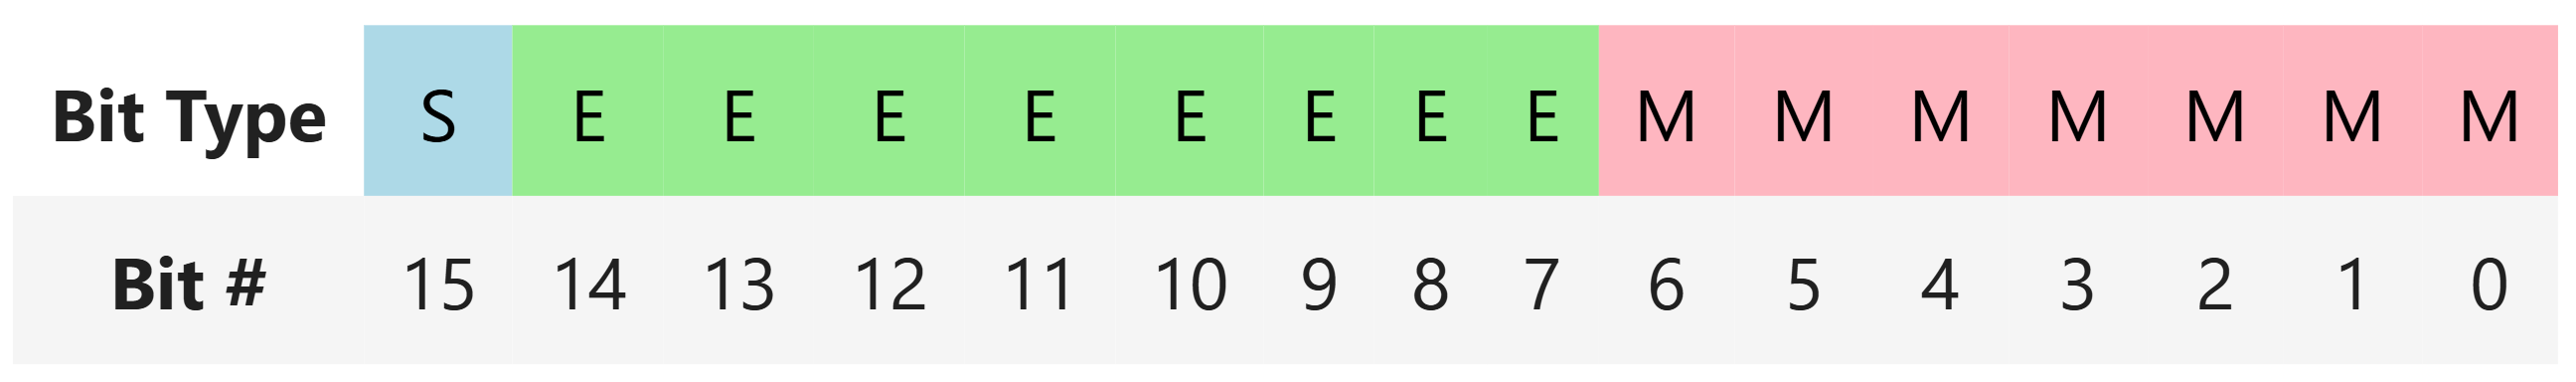
\includegraphics[width=0.75\linewidth]{q1_checkpoint/bf16.png}
    \caption{BF16 sign, exponent, and mantissa breakdown}
    \label{fig:BF16}
\end{figure}

BF16, or Brain Floating-Point 16, is widely adopted in machine learning for its ability to retain the same dynamic range as FP32 while reducing memory usage and computational requirements by using a lower precision mantissa. This format uses 8 bits for the exponent (like FP32) and 7 bits for the mantissa (compared to FP32's 23 bits), as shown in Figure \ref{fig:BF16}, making it effective for deep learning tasks with minimal accuracy loss. By sharing the same number of exponent bits as FP32, BF16 enables stable training and inference for large models like LLaMA, Qwen, and Phi, despite its reduced mantissa size.

The format follows this equation for normal numbers:
$$ (-1)^{\textstyle{sign}} × 2^{\text{exp} - 127} × (1 + \frac{\text{mantissa}}{2^7}) $$

And for subnormal numbers (when exponent = 0):
$$ (-1)^{\textstyle{sign}} × 2^{-126} × (0 + \frac{\text{mantissa}}{2^7}) $$

\subsubsection*{Floating Point Multiplication}

Before we dive into the \lmul algorithm, it's important to understand standard floating-point multiplication. As we discussed, a floating point number can be represented with a sign bit $s$, exponent bits $e$, bias $b$, and mantissa bits $m$ where the value $v$ is calculated as:

$$
v = (-1)^{\textstyle s} \times 2^{\textstyle (e-b)} \times (1+m) \\
$$

To add two floats together,

To multiply two floats together, we use the following equation:

\begin{align*}
    Mul(x, y) &= (1 + x_m) \cdot 2^{x_e} \cdot (1 + y_m) \cdot 2^{y_e} \\
    &= (1 + x_m + y_m + x_m \cdot y_m) \cdot 2^{x_e + y_e} 
\end{align*}

Incorporating our sign bit, we have:

\begin{equation*}
    p = (s_1 \oplus s_2) \times 2^{\textstyle (e_1+e_2-2b)} \times (1+m_1+m_2+m_1 \times m_2)
\end{equation*}

Because the exponents are biased, we must subtract the bias twice to compute the unbiased exponent, otherwise, the bias is counted twice:

\begin{align*}
    e_{\text{unbiased}} &= e_1 + e_2 - 2b \\
    e_{\text{bits}} &= e_{\text{unbiased}} + b \\
    e_{\text{bits}} &= e_1 + e_2 - b
\end{align*}

\subsubsection*{The Linear-Complexity Multiplication Algorithm (\lmul)}

In comparison, the core idea of the \lmul algorithm is that we can eliminate the multiplication of $m_1 \times m_2$ by approximating it with a term $L(M)$ where $M$ is the number of mantissa bits. The $L$ function is defined as:

\begin{equation*}
 L(M) =
   \left\{\begin{array}{lr}
       M, & M \le 3 \\
       3, & M = 4 \\
       4, & M > 4 \\
    \end{array}\right.
 \end{equation*}

And the multiplication algorithm becomes:  
$$
(s_1 \oplus s_2) \times 2^{\textstyle (e_1+e_2-b)} \times (1+m_1+m_2+L(M))
$$

In practice, we can perform this algorithm by taking the $XOR$, performing a bitwise addition on the combined exponent and mantissa parts, adding the $L(M)$ term, and subtracting the bias bit shifted to the left to align with the exponent part. This enables us to skip the normalization step since the mantissa carry is automatically added to the exponent.

\vspace{1em}

\textbf{A Note on Subnormals}

For now, we are not handling subnormal numbers and treating them as 0. We will handle them later. We think this approach is correct, but are still working on it:

A subnormal number is represented with exponent $e=0$ and defined as:
$$ (-1)^s \times 2^{e+1-b} \times (0+m) $$

Multiplying two subnormal numbers will always underflow to 0, but multiplying a normal $\times$ subnormal can result in 0, subnormal, or normal. The multiplication of a normal number $x$ and subnormal number $y$ with $y_e=0$ looks like:

$$
(x_s \oplus y_s) \times 2^{\textstyle (x_e+1-b)} \times (0+y_m)(1+x_m) \\
$$

The mantissa portion becomes: $(0 + y_m + y_m x_m) = (y_m + L(M))$

\subsubsection*{Systolic Array}
There are a variety of ways to perform matrix multiplication, but our specific implementation uses a systolic array.  The concept for the systolic array involves an array of processing elements which have data passed between them.  A processing element contains a multiply module (in our case this is the \lmul module) and an accumulate module.  the processing element recieves a number from the top and left, multiplies them, then adds them to a contained total.  The numbers are then passed to processing elements down and right.  This structure allows for a systolic array to perform matrix multiplication by having two matrices passed in row by row.  The data is multiplied when it intersects in processing elements, similarly to how matrix multiplication is performed by hand.  Once all the data is passed through, the accumulated sums in each processing element can be read out to view the multiplied matrix.  This diagram showcases the systolic array process, where data is fed in row by row, and where it intersects in processing elements it is multiplied and accumulated \citep{5x5systolic}. 

\pagebreak
\begin{figure}[htbp]
    \centering
    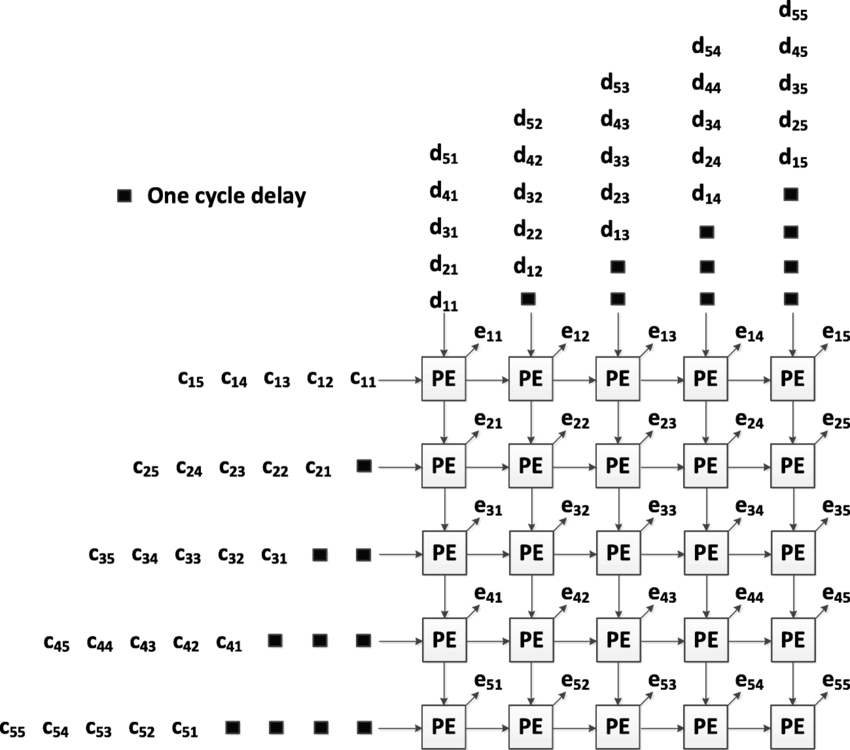
\includegraphics[width=14cm]{55-Systolic-array-architecture.png}
    \label{fig:Systolic array diagram}
\end{figure}

\subsubsection*{Utilizing PyRTL Implementation}

Our team works with PyRTL, a Python-based hardware description language (HDL) designed to simplify digital hardware design and prototyping. Combining the flexibility of Python with low-level control over digital logic, PyRTL serves as a bridge between traditional HDLs (e.g., Verilog) and High-Level Synthesis (HLS) tools \citep{clow2017pythonic}.

\textbf{Key Features}
\begin{itemize}
    \item \textbf{Ease of Use}: PyRTL leverages Python's syntax, including loops and comprehensions, to make hardware description intuitive and compact.
    \item \textbf{Intermediate Representation (IR)}: PyRTL provides a versatile IR for simulation, optimization, and conversion to other formats like Verilog.
    \item \textbf{Functional Simulation}: PyRTL supports built-in functional simulation for rapid design verification.
    \item \textbf{Integration with Physical Platforms}: PyRTL demonstrates compatibility with platforms like Xilinx PYNQ for deploying designs on SoCs.
    \item \textbf{Pedagogical Utility}: PyRTL simplifies hardware modeling and testing, making it accessible for teaching and learning.
\end{itemize}


\subsection{Verilog Implementation}
In conjunction with our experiments in implementing the Linear-Complexity Multiplication Algorithm module in simulation for PyRTL, we also used Xilinx’s Vivado to write the Verilog code for a systolic array using the \lmul algorithm.  Verilog is a lower-level HDL (hardware description language) that is used to specify the design of hardware.  We write Verilog code, then the Vivado program synthesizes the code into a runnable bitstream for an FPGA to run.  The language is similar to C++, but has its own features that aid Vivado in synthesizing the code. 

\subsubsection*{Design goals}
For this module (referred to as an IP core), our goal was to develop a 2x2 systolic array that multiplies two 2x2 matrices of BF16 numbers that utilize the \lmul algorithm in its multiply and accumulate unit. We designed the various IP cores from scratch so that as we progress this project further we will be able to optimize the design for the best performance.  As discussed above, we chose to store our floats in the BF16 format, which means data is passed through the systolic array and various processing elements in the form of 16-bit connections.

\subsection{PyRTL Implementation}

To validate our designs before FPGA deployment, we implemented our circuits using PyRTL, a Python framework for register-transfer level design. Through PyRTL, we created and tested digital circuits with visualizations and simulations. One of the key portions of our implementations was the nand-gate circuits that we attached at the end, which are indicative of power usage. We developed three key implementations: a standard floating-point multiplier, a linear-complexity multiplier (\lmul), and a floating-point adder. We plan on running test cases of (input1, input2) pairs through both of our multiplication algorithms. The IEEE-754 implementation should see no difference with the actual answer, however, we expect to see small differences with \lmul.

\subsubsection{Basic Components}

Our implementations share several fundamental components for handling BFloat16 numbers:

\begin{itemize}
    \item \textbf{Sign Extraction}: Isolates the sign bit from the 16-bit input
    \item \textbf{Exponent Extraction}: Extracts the 8-bit exponent field
    \item \textbf{Mantissa Extraction}: Retrieves the 7-bit mantissa and adds the implicit leading 1
\end{itemize}

\subsubsection{Standard Floating-Point Multiplier}

The standard multiplier implementation follows the IEEE-754 multiplication algorithm, structured in four pipeline stages. These pipeline stages were derived from the following paper \citep{niknia2024asic}.

\begin{enumerate}
    \item \textbf{Stage 1 (Input Processing)}: Extracts the components (sign, exponent, mantissa) from both input numbers.
    
    \item \textbf{Stage 2 (Core Computation)}:
    \begin{itemize}
        \item Computes output sign using XOR of input signs
        \item Adds exponents using carry-lookahead adder
        \item Multiplies mantissas using a carry-save tree multiplier
    \end{itemize}
    
    \item \textbf{Stage 3 (Normalization Preparation)}:
    \begin{itemize}
        \item Implements leading zero detection using a binary tree structure
        \item Adjusts exponent by removing bias (subtracting 127)
    \end{itemize}
    
    \item \textbf{Stage 4 (Post-Processing)}:
    \begin{itemize}
        \item Normalizes the mantissa product
        \item Implements round-to-nearest-even logic
        \item Adjusts final exponent based on normalization and rounding
    \end{itemize}
\end{enumerate}

\subsubsection{Linear-Complexity Multiplier (\lmul)}

The \lmul implementation consists of three pipeline stages, optimized for hardware efficiency by reducing multiplication complexity to linear operations:

\begin{enumerate}
    \item \textbf{Stage 1 (Input Registration): }
    \begin{itemize}
        \item Registers input operands (fp\_a, fp\_b)
        \item Prepares values for exponent/mantissa manipulation
        \item Pipeline depth is optimized with minimal latency between input and first operation
    \end{itemize}
    \item \textbf{Stage 2 (Core Computation): }
    \begin{itemize}
        \item Computes result sign using XOR of input signs
        \item Performs the key \lmul operation by adding the exp\_mantissa fields
        \item Uses a carry-save adder tree followed by Kogge-Stone adder for fast addition
        \item Subtracts the format-specific offset using a pre-computed constant
    \end{itemize}
    \item \textbf{Stage 3 (Output Formatting): }
    \begin{itemize}
        \item Implements overflow/underflow detection using carry and MSB
        \item Selects appropriate output value using a multiplexer: 
        \begin{itemize}
            \item Underflow case: Returns zero (0x00)
            \item Normal case: Uses computed sum
            \item Overflow case: Returns format-specific maximum value
        \end{itemize}
        \item Concatenates final sign and result bits
    \end{itemize}
\end{enumerate}
The pipeline achieves efficiency through several optimizations:

\begin{itemize}
    \item Eliminates costly mantissa multiplication by converting to addition in log domain
    \item Uses fast adder implementations (carry-save + Kogge-Stone) to minimize critical path
    \item Handles special cases through simple multiplexer-based selection
    \item Maintains numerical stability by properly handling overflow/underflow conditions
\end{itemize}
The implementation supports different floating point formats (FP8, BF16) through parameterization of the exponent and mantissa bit widths, making it flexible for various precision requirements.

 

\subsubsection{Floating-Point Adder}

The floating-point adder implementation consists of five pipeline stages:

\begin{enumerate}
    \item \textbf{Input Parsing}: Extracts sign, exponent, and mantissa components
    
    \item \textbf{Exponent Alignment}:
    \begin{itemize}
        \item Calculates exponent difference
        \item Determines larger exponent
        \item Prepares for mantissa alignment
    \end{itemize}
    
    \item \textbf{Mantissa Alignment}:
    \begin{itemize}
        \item Implements right-shift logic for smaller mantissa
        \item Generates sticky, guard, and round bits
    \end{itemize}
    
    \item \textbf{Addition/Subtraction}:
    \begin{itemize}
        \item Performs mantissa addition or subtraction based on signs
        \item Implements leading zero detection for normalization
    \end{itemize}
    
    \item \textbf{Normalization and Rounding}:
    \begin{itemize}
        \item Normalizes result using leading zero count
        \item Implements round-to-nearest-even logic
        \item Adjusts final exponent
    \end{itemize}
\end{enumerate}

\subsubsection{Pipeline Implementation}

We developed a pipeline framework using PyRTL's Register class to manage sequential logic. The \texttt{SimplePipeline} base class was used to generate our pipelines with automatic register generation and stage management. This was essentially a utility class allowing us to experiment with different pipeline depths and configurations and managing our timing relationships for us.

\section{Results}

\begin{table}[htbp]
    \caption{BF16 \lmul Basic Analysis}
    \label{tab:bf16_lmul}
    \resizebox{1\linewidth}{!}{\begin{tabular}{|c|c|c|c|c|c|c|c|}
\hline
Step & Input A & Input B & Expected Result & Actual IEEE & Actual LMUL & Diff IEEE & Diff LMUL \\
\hline
0 & $9.9945 \times 10^{-4}$ & $9.9945 \times 10^{-4}$ & $9.9838 \times 10^{-7}$ & $9.9838 \times 10^{-7}$ & $1.0580 \times 10^{-6}$ & 0 & $5.9605 \times 10^{-8}$ \\
\hline
1 & $9.9945 \times 10^{-4}$ & $1.0010 \times 10^{-2}$ & $1.0014 \times 10^{-5}$ & $1.0014 \times 10^{-5}$ & $1.0431 \times 10^{-5}$ & 0 & $4.1723 \times 10^{-7}$ \\
\hline
2 & $9.9945 \times 10^{-4}$ & $1.0010 \times 10^{-1}$ & $1.0014 \times 10^{-4}$ & $1.0014 \times 10^{-4}$ & $1.0300 \times 10^{-4}$ & 0 & $2.8610 \times 10^{-6}$ \\
\hline
3 & $9.9945 \times 10^{-4}$ & 1.0 & $9.9945 \times 10^{-4}$ & $9.9945 \times 10^{-4}$ & $1.0605 \times 10^{-3}$ & 0 & $6.1035 \times 10^{-5}$ \\
\hline
4 & $1.0010 \times 10^{-2}$ & $1.0010 \times 10^{-2}$ & $1.0014 \times 10^{-4}$ & $1.0014 \times 10^{-4}$ & $9.9182 \times 10^{-5}$ & 0 & $-9.5367 \times 10^{-7}$ \\
\hline
5 & $1.0010 \times 10^{-2}$ & $1.0010 \times 10^{-1}$ & $9.9945 \times 10^{-4}$ & $9.9945 \times 10^{-4}$ & $9.4986 \times 10^{-4}$ & 0 & $-4.9591 \times 10^{-5}$ \\
\hline
6 & $1.0010 \times 10^{-2}$ & 1.0 & $1.0010 \times 10^{-2}$ & $1.0010 \times 10^{-2}$ & $1.0498 \times 10^{-2}$ & 0 & $4.8828 \times 10^{-4}$ \\
\hline
7 & $1.0010 \times 10^{-1}$ & $1.0010 \times 10^{-1}$ & $1.0010 \times 10^{-2}$ & $1.0010 \times 10^{-2}$ & $9.8877 \times 10^{-3}$ & 0 & $-1.2207 \times 10^{-4}$ \\
\hline
8 & $1.0010 \times 10^{-1}$ & 1.0 & $1.0010 \times 10^{-1}$ & $1.0010 \times 10^{-1}$ & $1.0400 \times 10^{-1}$ & 0 & $3.9063 \times 10^{-3}$ \\
\hline
9 & 1.0 & 1.0 & 1.0 & 1.0 & $1.0625$ & 0 & $6.2500 \times 10^{-2}$ \\
\hline
\end{tabular}}
\end{table}

\subsection{Understanding \lmul Accuracy: Initial Interpretations with FP8}

Since there are not that many total representable values using the FP8 format (max 256), we can plot a heatmap of the error for every combination of multiplications:
\pagebreak
\begin{figure}[htbp]
    \centering
    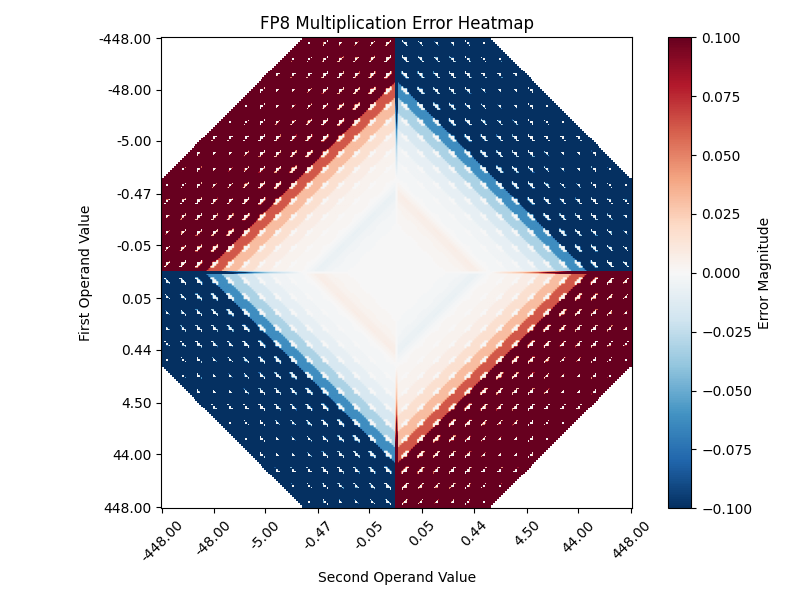
\includegraphics[width=.65\linewidth]{q1_checkpoint/fp8_multiplication_error.png}
    \label{fig:fp8_multiplication_error}
\end{figure}

From Figure \ref{fig:fp8_multiplication_error}, we can see that the largest magnitude errors generally occur when multiplying a small and large number together. Generally, errors tend to be lower when multiplying smaller values, which is good since the application of this algorithm is for machine learning models whose weights tend to be in well-defined ranges like $[0,1]$ or $[-1,1]$.

Now let's compare to the basic \lmul algorithm:

\begin{figure}[htbp]
    \centering
    \includegraphics[width=\linewidth]{q1_checkpoint/basic_lmul_normalxsubnormal.png}
    \label{fig:basic_lmul_normalxsubnormal}
\end{figure}

And our modified algorithm to handle subnormals:
\pagebreak
\begin{figure}[htbp]
    \centering
    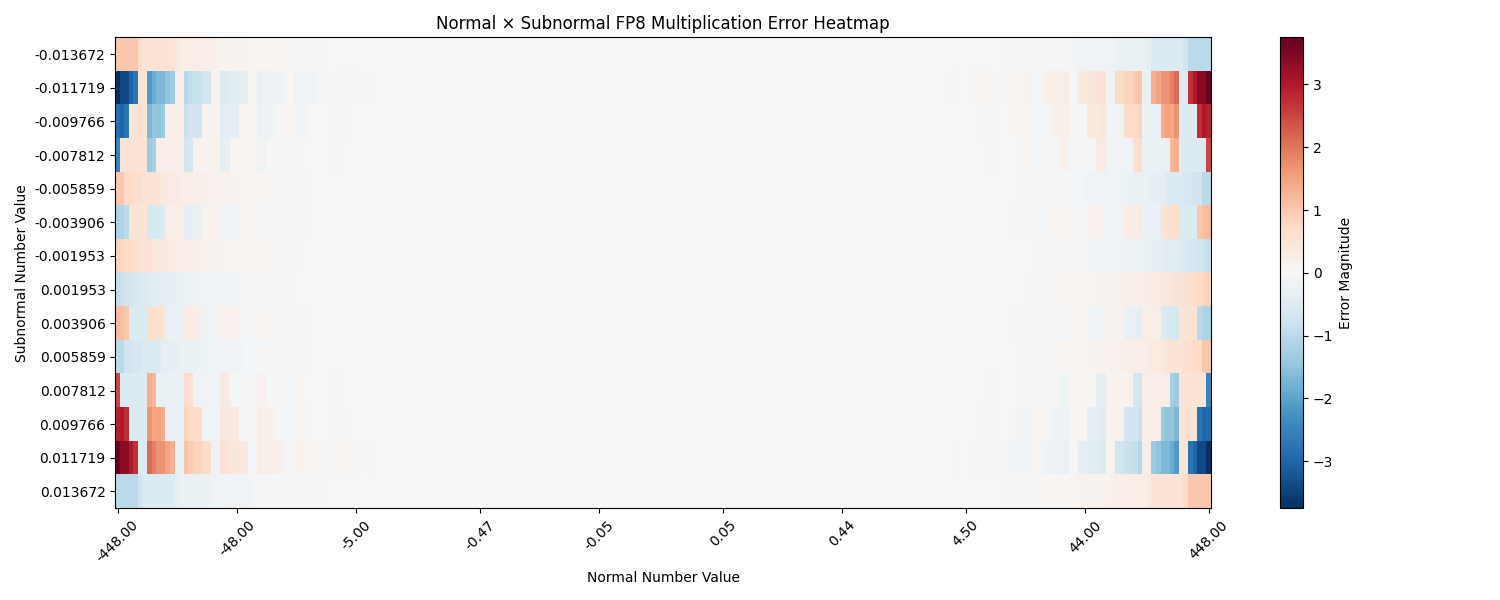
\includegraphics[width=\linewidth]{q1_checkpoint/optimized_lmul_normalxsubnormal.png}
    \label{fig:optimized_lmul_normalxsubnormal}
\end{figure}

\subsection{Verilog}

\begin{figure}[htbp]
    \centering
    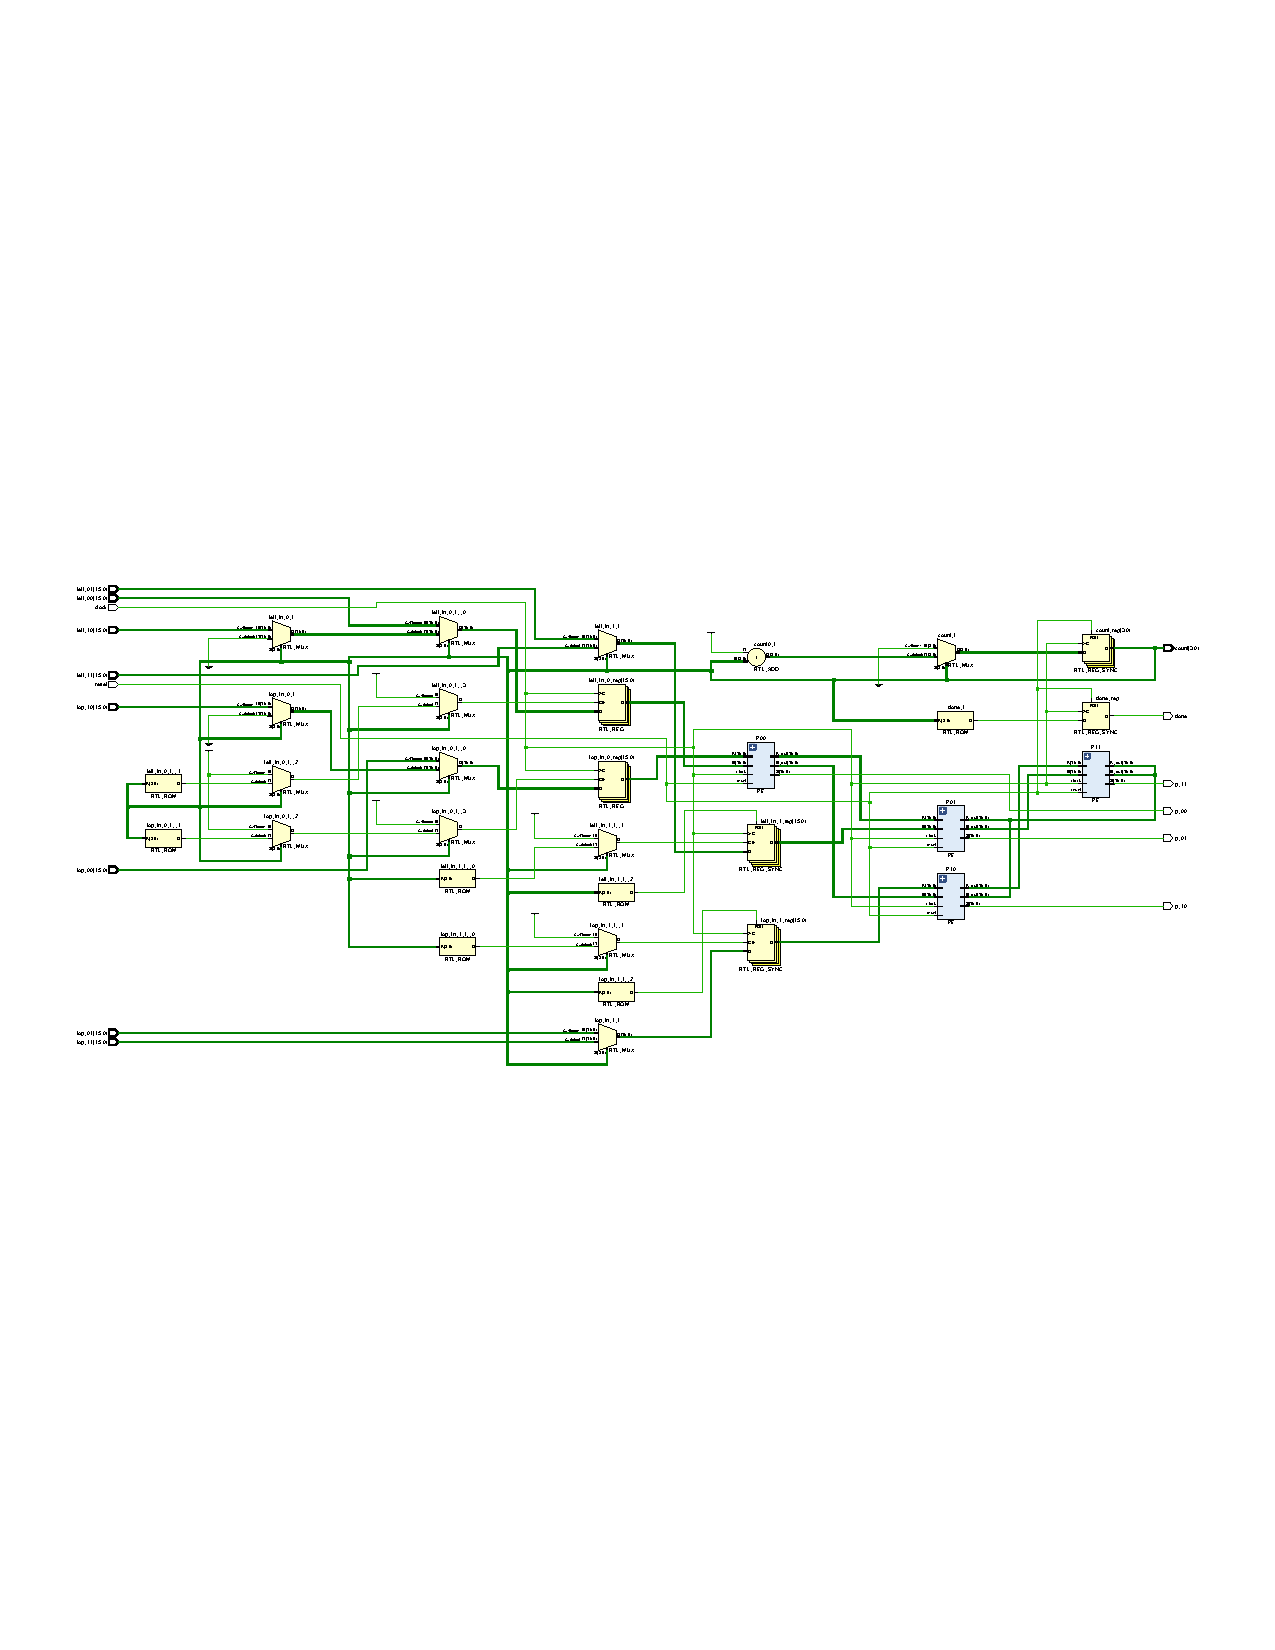
\includegraphics[clip, trim=0.5cm 9.5cm 0.5cm 9.5cm, width=1.00\textwidth]{Verilog Schematics/systolic.pdf}
    \caption{The full schematic for the 2x2 systolic array}
    \label{fig:PE}
\end{figure}

This is the diagram of the schematic generated for the 2x2 systolic array, from the input data to the actual processing element array, and the control logic.  The IP core takes the two 2x2 matrices of BF16 floats, a reset pin, and a clock pin.  The outputs are read from each processing element, in the form of 4 16 bit outputs.  It operates in three clock cycles once all the data is present to the inputs, and reports the done pin after three cycles.  

The IP core is divided into multiple sections, the input registers, the control logic, and the processing elements.  As with the behavior of a systolic array, the data is passed into the array as rows from the top and left.  This is represented in the schematic as the four yellow rectangles in the middle of the diagram.  These blocks receive data from the input pins in accordance with the control logic and then send them into the processing element array.  This switching is controlled by the field of trapezoids, which represent multiplexers that feed the inputs into the correct registers.  This is due to the systolic array taking in elements in sequence while the data is presented to the IP core all at once.  

The five elements in the top right represent the control logic, housing the counter circuit.  When the clock signal is applied it counts from zero to two, then resets when the reset signal is applied.  The reset signal also resets all the internal registers and the processing elements.  The control logic then switches the various multiplexers which determine where the inputs are placed for processing.

Finally, the staged data is passed into the 2x2 matrix of processing elements, represented by the grey blocks on the right.  Each processing element contains its own registers, so the output of the systolic array IP core is read directly from each processing element out.  The processing elements are connected down and right, with processing element 0, 0 connected to the top 0 and left 0 register, processing element 0, 1 connected to the top pass-through of processing element 0, 0, and the left 1 register.  This continues through the other two, but the key behavior here is that each processing element outputs its top input down and its left input right, such that the next processing element receives it.  But the pass-through occurs with a delay of one cycle, so data flows across and down the processing elements, where it is then multiplied and accumulated in each processing element.

\subsubsection*{Processing Element}

\begin{figure}[h]
    \centering
    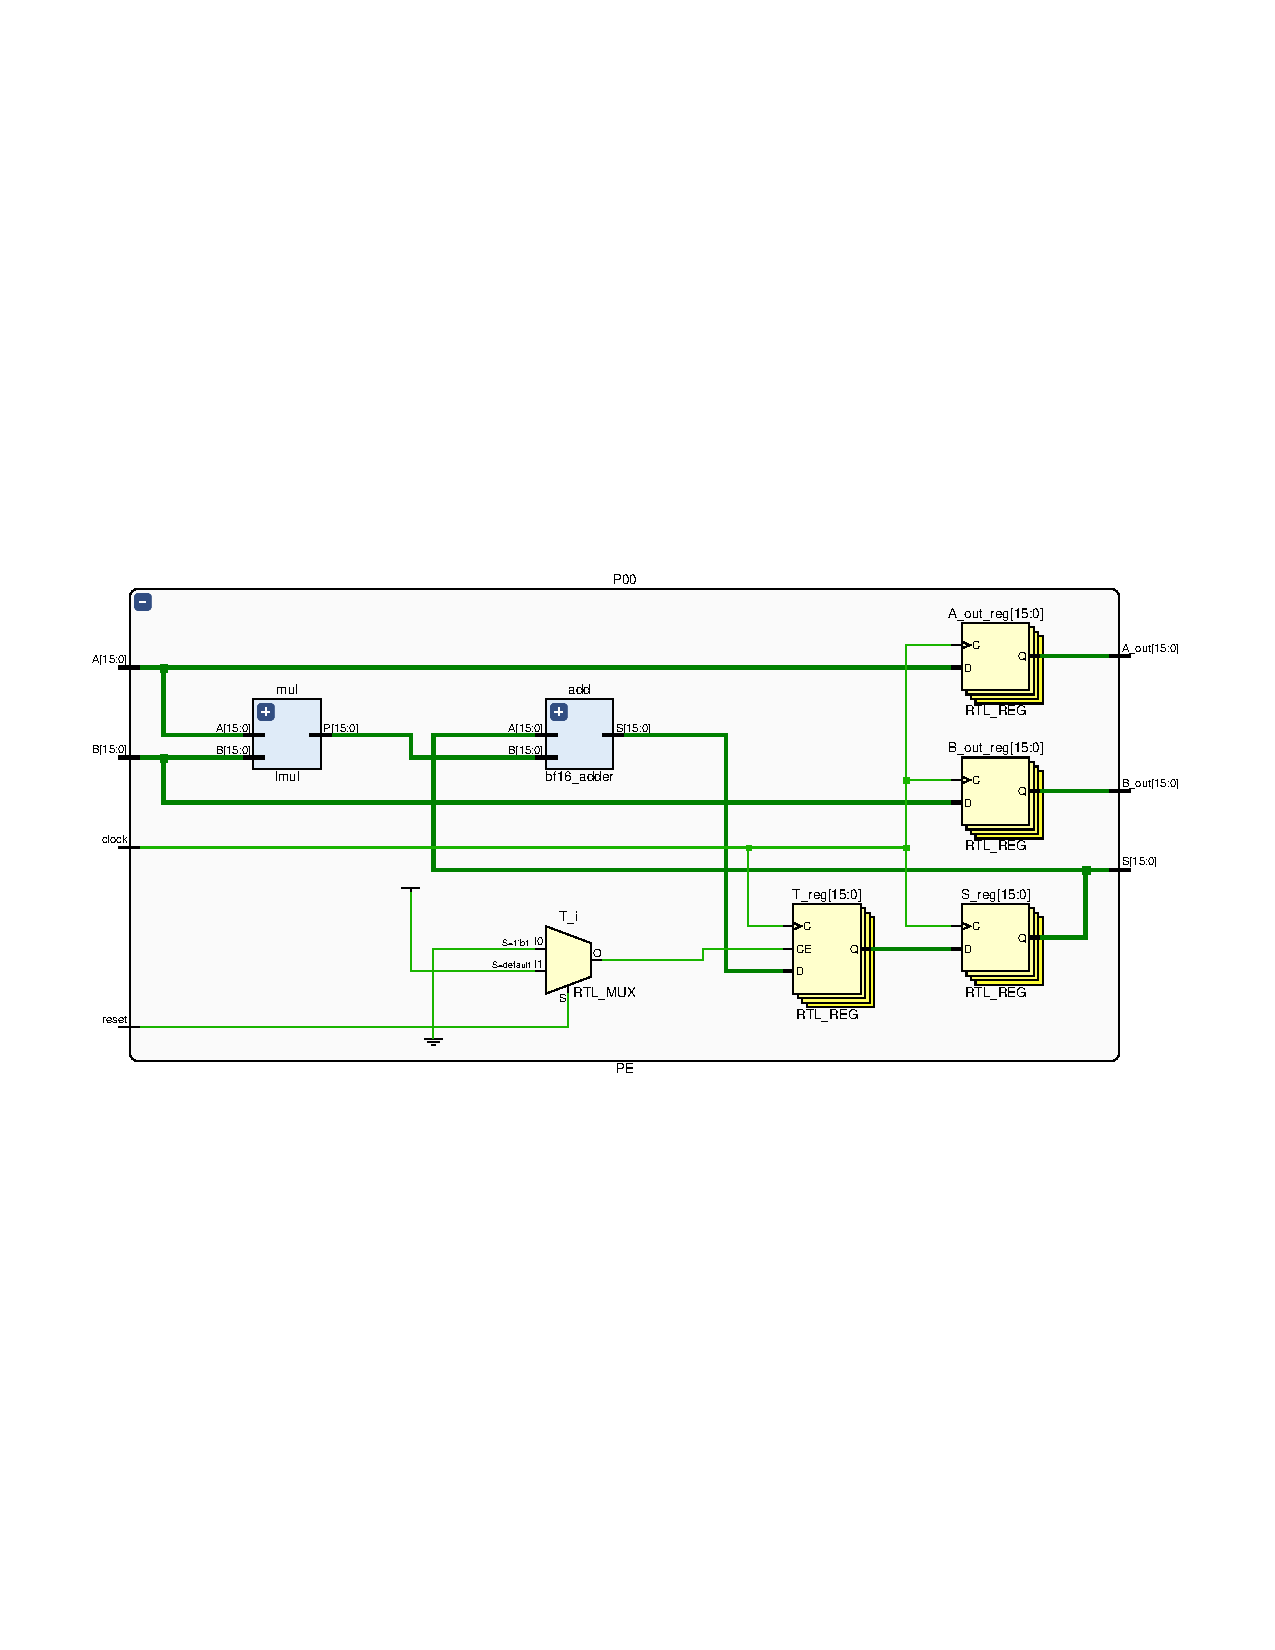
\includegraphics[clip, trim=0.5cm 9cm 0.5cm 9cm, width=1.00\textwidth]{Verilog Schematics/PE.pdf}
    \caption{The schematic for the processing element}
    \label{fig:adder}
\end{figure}

Each processing element is made up of a multiply unit, an adder unit, and the data registers.  It takes in two BF16 numbers, A and B, as well as a clock and reset signal.  When the Processing element receives the clock signal it passes the inputs A and B through the \lmul module, then passes the result from the \lmul module to the adder.  The value is added to the existing accumulated value stored within the 16-bit S register.  The new sum is put into the 16-bit T register, then shifted into the S register as the new accumulated sum.  Alongside the math operation, the A and B values are written into the 16-bit A out and B out registers, which present the values to the adjacent processing elements to allow data to flow through the systolic array.  


\subsubsection*{BF16 Adder}

\begin{figure}[h]
    \centering
    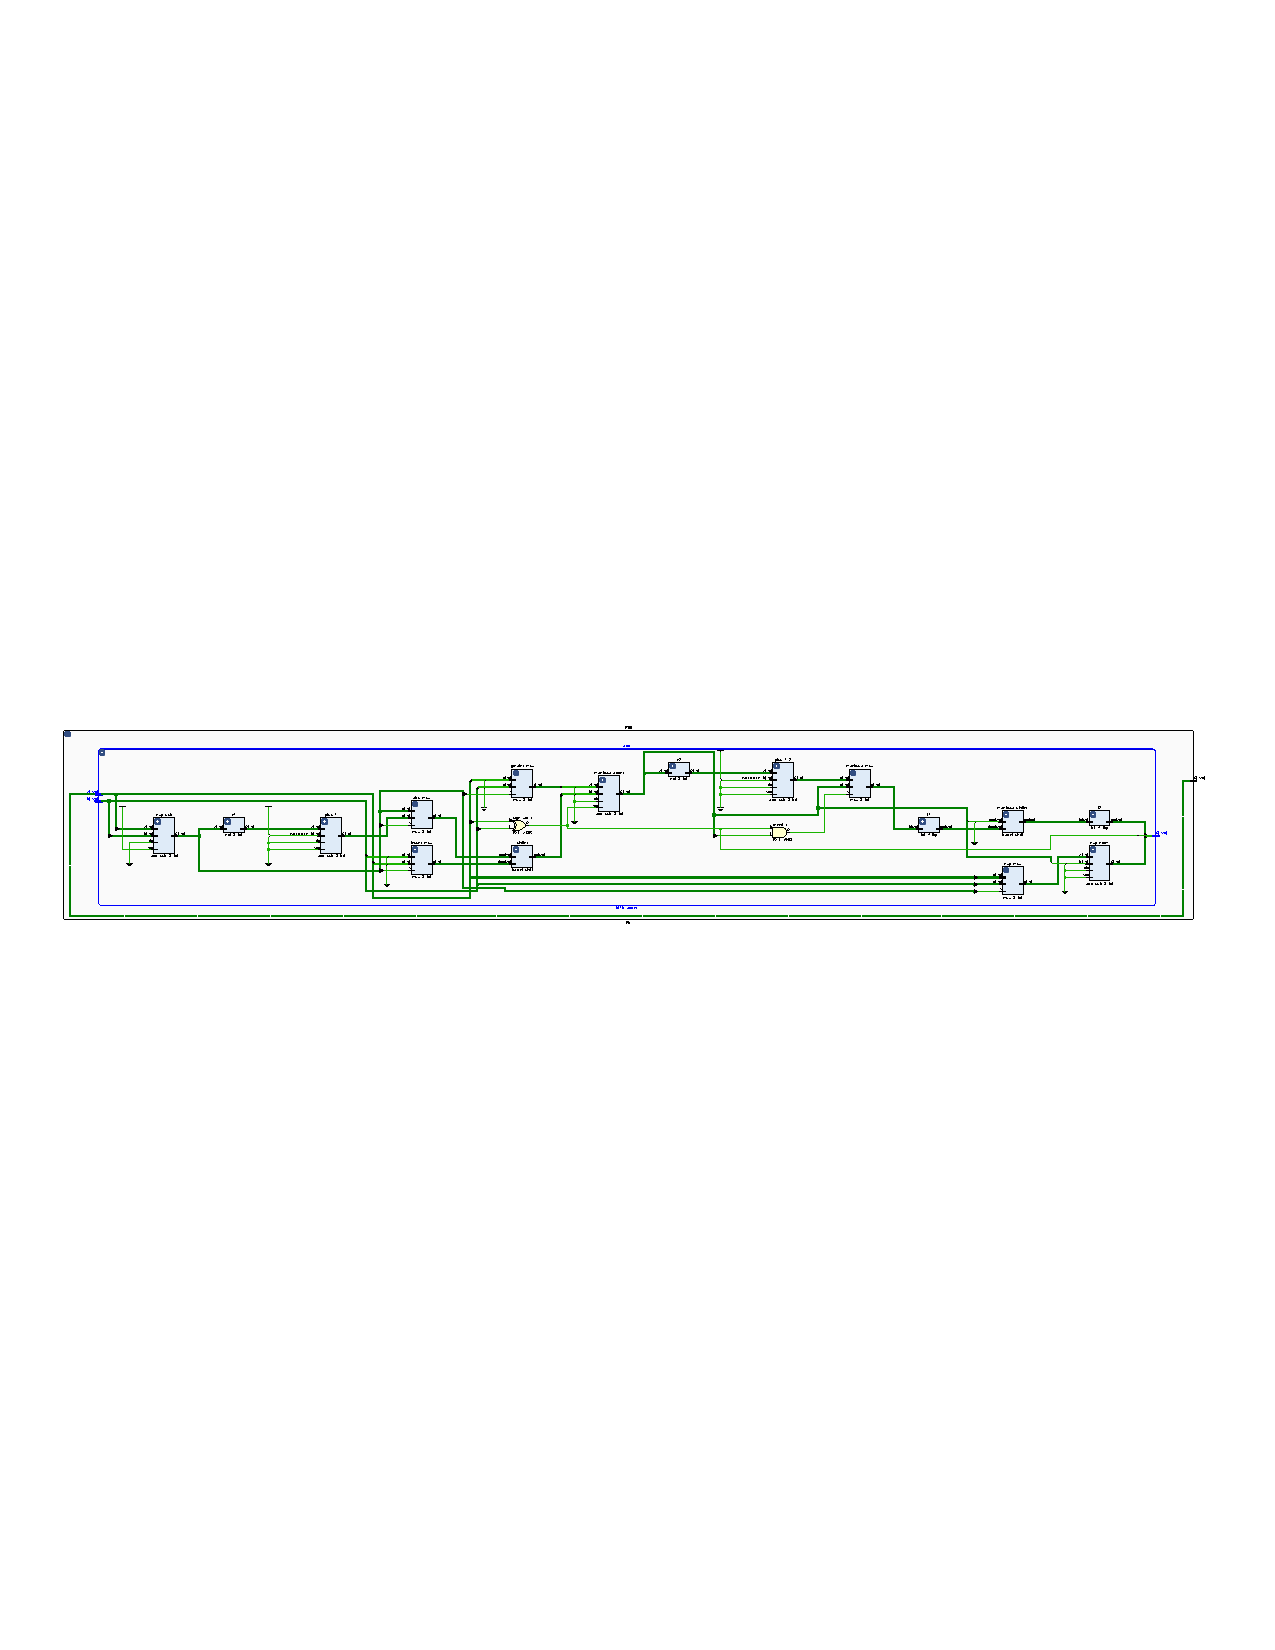
\includegraphics[clip, trim=0.5cm 11cm 0.5cm 11cm, width=1.00\textwidth]{Verilog Schematics/adder.pdf}
    \caption{The schematic for the BF16 adder}
    \label{fig:systolic}
\end{figure}

This chain of gates represents a BF16 adder.  Originally we expected the multiply unit of the processing element to be the most complex, but the simplification of the multiplication algorithm offered by the \lmul algorithm simplified it greatly, making the addition circuit more complex.  This is mainly due to normalization, where floating point numbers cannot be directly added due to the differing exponents. Instead, the smaller number must have its mantissa bits shifted so that the exponents are added, then the number can be added and finally normalized back down in case of an overflow.

The beginning of the diagram consists of a subtractor module to determine which exponent is smaller, using the sign bit of the subtraction to determine which is smaller.  That information is used to load the mantissas using multiplexers so that the mantissas can be added, though the smaller one must pass through a barrel shifter shifting by the difference in the exponent subtraction.  After the mantissa addition, the value has to be normalized, and the exponent adjusted accordingly.

\subsubsection*{\lmul}

The \lmul module is surprisingly simple, but this is what gives it the performance boost over regular multiplication we are looking for.  As we have described the behavior above the module takes in two BF16 numbers A and B, and returns a 16bf number P.  The module simply adds them together, then subtracts the offset term 16'b0011111101111000.  This term is actually two distinct terms, representing the addition of the offset as defined by the \lmul algorithm, as well as the correction for the bias of floating point.  This is combined into a single term, then subtracted for the output.  The rest of the module is the check module, which looks to see if any of the number exponents are all zero, and if so returns zero instead of the product, effectively rounding subnormal values down to zero.

\begin{figure}[htbp]
    \centering
    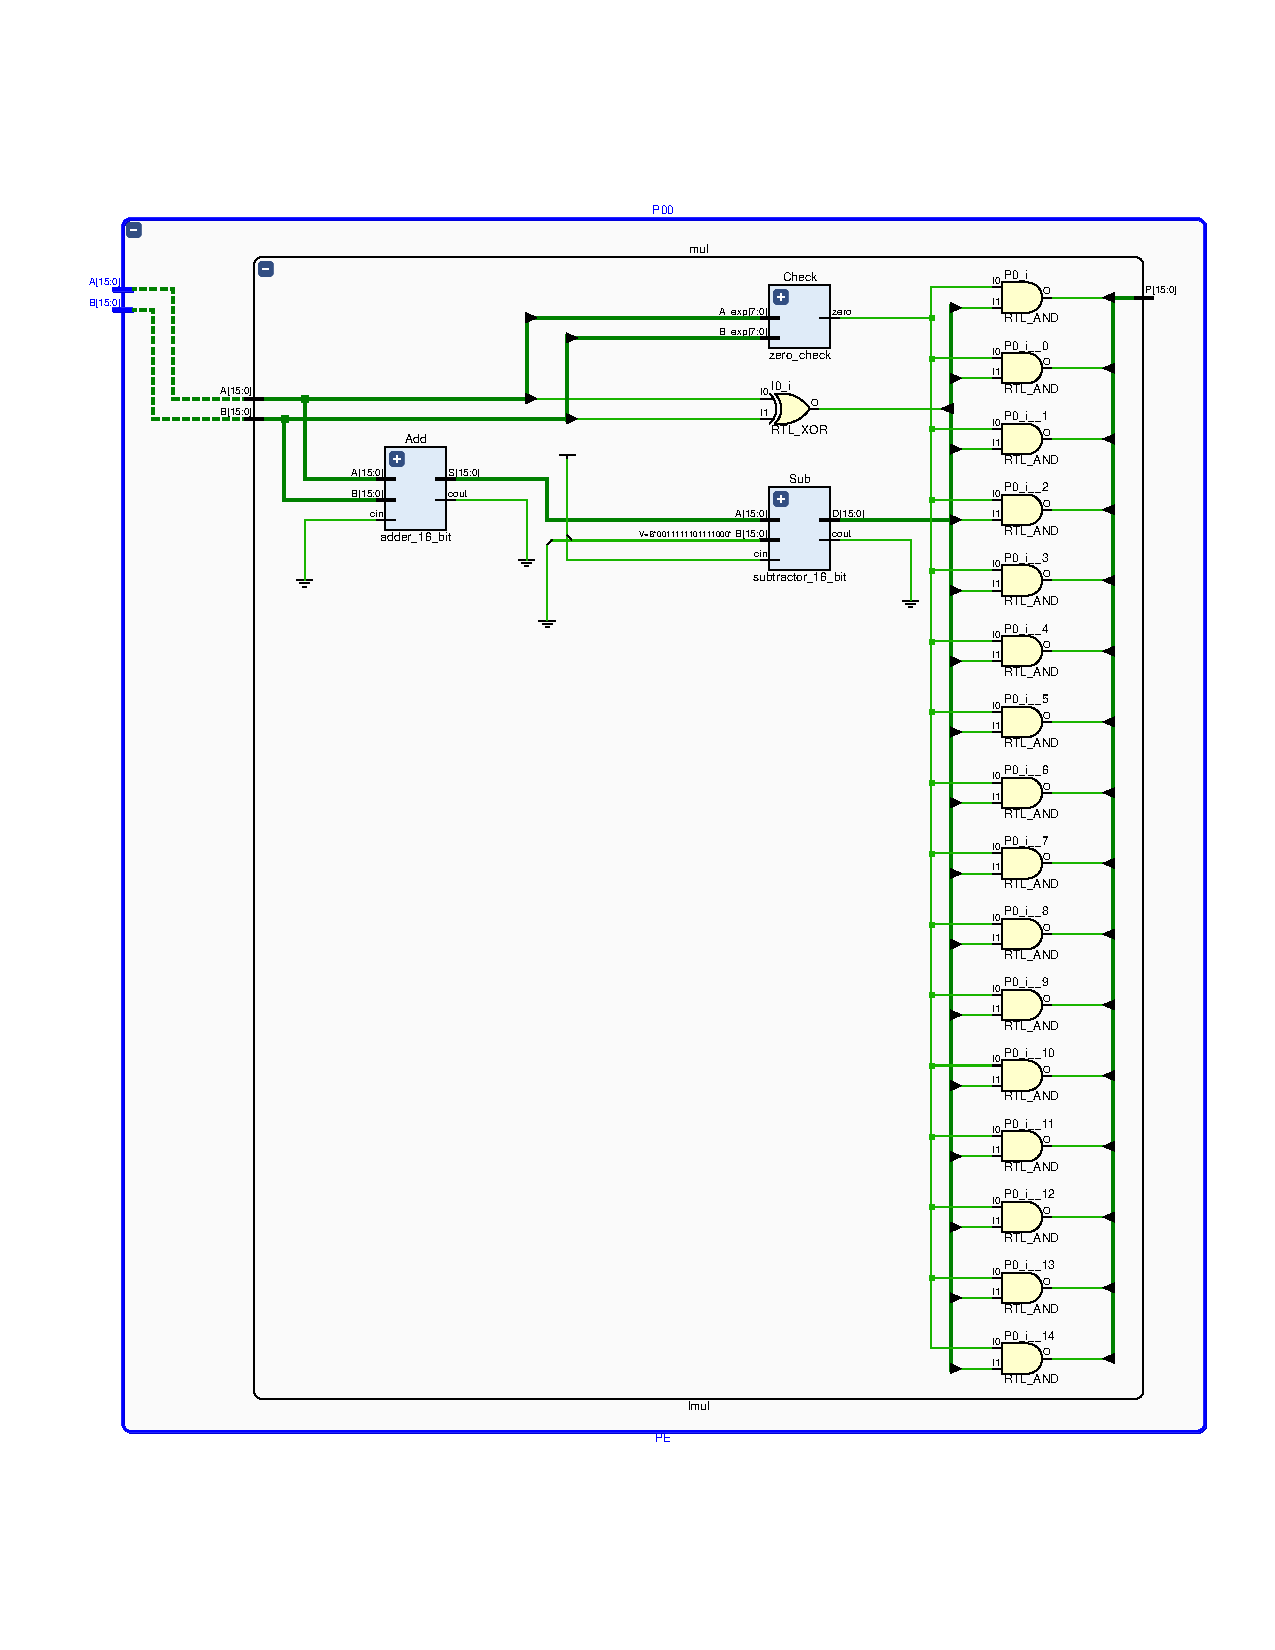
\includegraphics[clip, trim=0.5cm 3cm 0.5cm 3cm, width=.85\textwidth]{Verilog Schematics/lmul.pdf}
    \caption{The schematic for the \lmul module}
    \label{fig:lmul}
\end{figure}



\section{Discussion}

\subsection{Difficulties with Software}
Though we were able to generate a systolic array in both PyRTL and Vivado the implementation was slow and difficult.  Writing code at the gate level, especially in Verilog was challenging, and Vivado being a clunky program did not help matters.  Hours were spent on implementing operations as simple as addition, and learning the unique design philosophies required us to change how we thought about coding.  This has manifested in our plans for quarter two, where we will be dropping Verilog build path in favor of dedicating all of our work to the PyRTL approach.  We will still be able to import the Verilog we have already written, but hopefully switching to a higher level language will allow us to progress our project quicker and more efficiently, while allowing to build on our work more easily as well.

\subsection{PyRTL Implementation Results}

Our PyRTL implementation validated the key findings from the \citep{luo2024addition} paper regarding the \lmul algorithm. As expected, our hardware implementation showed that \lmul produced small but consistent errors compared to standard floating-point multiplication. These errors primarily manifested when multiplying numbers of significantly different magnitudes, but remained minimal for values within typical neural network parameter ranges.

The paper's authors highlighted that the true challenge would lie in hardware implementation rather than theoretical development – our work directly addressed this challenge by creating a working RTL design. We successfully implemented both the standard floating-point multiplier and the \lmul algorithm in PyRTL, demonstrating that the theoretical simplifications do indeed translate to practical hardware designs. The most complex part of our implementation wasn't the \lmul algorithm itself, but rather the supporting floating-point infrastructure, particularly the addition circuit required for the final stage.

Importantly, our results align with the paper's assertion that these small accuracy differences are inconsequential for neural network performance. This opens up several exciting avenues for Quarter 2 exploration, particularly around systolic array implementations and potential FPGA deployments. Our successful PyRTL implementation serves as a proof-of-concept that the \lmul algorithm can be effectively translated to hardware, potentially leading to significant performance improvements in real-world neural network accelerators.


\subsection{Real World Obstacles}
We also faced a challenge in the available resources.  Hardware design is not like learning python, where there is limited open-source projects and tutorials available.  For example, working with Vivado involved using tutorials from four to six years ago, where the software looked and behaved radically differently, and trying to work from there.  We also originally wanted to deploy our module to a physical ASIC, but we were faced with price tags of tens of thousands of dollars to get a chip physically created.  We also have limited access to development tools as most are closed-source and closely guarded by their respective companies.

%%%%%%%%%%%%%%%%%%%%%%%%%%%%%%%%%%%%%
%% FIGURE U CAN COPY & PASTE
%%%%%%%%%%%%%%%%%%%%%%%%%%%%%%%%%%%%%
% \begin{figure}[htbp]
%     \centering
%     \includegraphics[width=\linewidth]{figure/basic_lmul_normalxsubnormal.png}
%     \caption{INSERT CAPTION HERE}
%     \label{fig:basic_lmul_normalxsubnormal}
% \end{figure}


\section{Conclusion}

When we look at a computer, it is easy to imagine it as a magical black box that takes in inputs and instructions then returns values, but it is important to consider the actual hardware within.  Something as simple as the multiplication operation, something we were all taught in early elementary school, is actually quite complex when expressed in hardware.  Unlike our elementary math classes where we can express multiplication with symbols like 2x3=6, we see the actual hardware storing numbers in a complex format and multiplying them taking a nontrivial algorithm to perform the operation.  And this project has shown that by utilizing a new multiplication algorithm we can vastly increase the performance of code that needs to multiply, and therefore speed up machine learning.



%%%%%%%%%%%%%%%%%%%%%%%%%%%%%%%%%%%%%%%%%%%%%%%%%%%%%%%%
%%%% Reference / Bibliography
%%%%%%%%%%%%%%%%%%%%%%%%%%%%%%%%%%%%%%%%%%%%%%%%%%%%%%%%

\makereference

\bibliography{reference}
\bibliographystyle{style/dsc180bibstyle}


%%%%%%%%%%%%%%%%%%%%%%%%%%%%%%%%%%%%%%%%%%%%%%%%%%%%%%%%
%%%% Appendix
%%%%%%%%%%%%%%%%%%%%%%%%%%%%%%%%%%%%%%%%%%%%%%%%%%%%%%%%

% \clearpage
% \makeappendix

% \subsection{Training Details}

% \subsection{Additional Figures}

% \subsection{Additional Tables}


\end{document}